\documentclass[notheorems, handout]{beamer}

\usetheme[numbers,totalnumbers,compress, nologo]{Statmod}
\usefonttheme[onlymath]{serif}
\setbeamertemplate{navigation symbols}{}
\setbeamertemplate{theorems}[numbered]
\setbeamertemplate{caption}[numbered]

\mode<handout> {
	\usepackage{pgfpages}
%	\setbeameroption{show notes}
%	\pgfpagesuselayout{2 on 1}[a4paper, border shrink=5mm]
	\setbeamercolor{note page}{bg=white}
	\setbeamercolor{note title}{bg=gray!10}
	\setbeamercolor{note date}{fg=gray!10}
}

\usepackage[utf8x]{inputenc}
\usepackage[T2A]{fontenc}
\usepackage[russian, english]{babel}
\usepackage{tikz}
\usepackage{ragged2e}

\newtheorem{corollary}{Следствие}
\newtheorem{theorem}{Теорема}
\newtheorem{remark}{Замечание}
\newtheorem{lemma}{Лемма}
\newtheorem{sentence}{Предложение}
\newtheorem{definition}{Определение}
\newtheorem{formulation}{Формулировка}
\newtheorem{statement}{Постановка}
\DeclareMathOperator{\R}{\mathbb{R}}
\DeclareMathOperator{\rank}{\mathrm{rank}}
\newcommand{\norm}[1]{\left\|#1\right\|}


\title[Задачи анализа временных рядов]{Задачи анализа временных рядов, теория метода «Анализ Сингулярного Спектра» SSA}

\author{Яковлев Денис Михайлович, гр.21.Б04-мм}

\institute[Санкт-Петербургский Государственный Университет]{%
	\small
	Санкт-Петербургский государственный университет\\
	Прикладная математика и информатика\\
	Вычислительная стохастика и статистические модели\\
	\vspace{1.25cm}
	3 курс (бак.) <<Производственная практика (научно-исследовательская работа)>>\\(Семестр 6)}

\date[Зачет]{Санкт-Петербург, 2024}

\subject{Talks}

\begin{document}
%	\begin{frame}[plain]
%		\titlepage
%		
%		\note{Научный руководитель  к.ф.-м.н., доцент Некруткин В.В.,\\
%			кафедра статистического моделирования\\\vspace*{2cm}\emph{Моя отметка за работу Дениса Яковлева -- 5  с минусом (очень хорошо).
%				5 за результат, минус – за стиль работы.
%		}}
%	\end{frame}
	\begin{frame}[plain]
		\titlepage
		
		\note{Научный руководитель  к.ф.-м.н., доцент Некруткин В.В.,\\
			кафедра статистического моделирования}
	\end{frame}
	
	%\section{Короткая тема}
	%\subsection{Общие слова}
	
%	\setbeameroption{show notes}
	
	\begin{frame}{Введение}
		\begin{itemize}
			\item Цель работы --- решение теоретических и прикладных задач анализа временных рядов с применением метода SSA. 
			\item Используемый метод --- SSA (Singular Spectrum Analysis), или <<Анализ Сингулярного Спектра>> (сокращенно, АСС).
			\item Задача --- исследование поведения ошибок восстановления ряда в асимптотическом случае.
		\end{itemize}
		%		Задача --- оценка ошибок восстановления ряда.
		%		Тут какое-то введение.
		%		Что за задача решается, какое метод используется, какая цель работы.
		
		\note{
			Целью этой  работы является решение теоретических и прикладных задач по анализу временных рядов с применением знаний о методе SSA (Singular Spectrum Analysis), или <<Анализ Сингулярного Спектра>> (сокращенно, АСС). Ознакомиться с методом АСС можно в \cite{GNZh01}, а в  \cite{Nekrutkin10} описывается теоретическая часть метода АСС. Общая задача состоит в том, чтобы оценить ошибки восстановления ряда.
		}
	\end{frame}
	%	\begin{frame}{Введение}
		%		
		%	\end{frame}
	%	
	%		\note{Кратко напомним о методе SSA}
	\begin{frame}{Обозначения}
		\begin{definition}[Сигнал]
			Вещественный сигнал $\mathrm{H} = (h_0, h_1, \dots, h_n, \dots)$, управляется линейной рекуррентной формулой  (ЛРФ) порядка~$d$
			\begin{gather*}
				h_n = \sum\limits_{k=1}^d a_kh_{n-k},\; n\geqslant d,\; a_d>0.
			\end{gather*} 
			$\mathrm{H}_N=(h_0,h_1,\dots,h_N)$.
		\end{definition} 
		\begin{definition}[Помеха]
			Помеха --- $\mathrm{E}_N=(e_0,\ldots, e_N)$.
		\end{definition}
		\note{
			Введём необходимые для постановки задачи определения и известные результаты. Начнём с определений. Рассматривается вещественный \emph{сигнал} $\mathrm{H}$, причем предполагается, что ряд управляется линейной
			рекуррентной формулой  (ЛРФ) порядка~$d$
			с $a_d>0$, которая является минимальной в том смысле, что  не существует ЛРФ меньшего порядка, управляющей рядом $\mathrm{H}$. Так как нас интересует использование метода SSA, будем рассматривать отрезки длины N.
			Кроме того, вводится \emph{помеха} $\mathrm{E}$, некоторый ряд из вещественных значений.
		}
	\end{frame}
	\begin{frame}{Обозначения}
		\begin{definition}[Траекторная матрица]
			Пусть $1\leqslant L < N$ --- длина окна, $K=N-L+1$. Тогда траекторной матрицей сигнала $\mathrm{H}_N = (h_0, h_1, \dots, h_N)$ называется матрица $\mathbf{H}$ размера $L\times K$ вида:
			\begin{equation*}
				\begin{pmatrix}
					h_0&h_1&h_2&\dots&h_{K-1}\\
					h_1&h_2&h_3&\dots&h_K\\
					h_2&h_3&h_4&\dots&h_{K+1}\\
					\vdots&\vdots&\vdots&\ddots&\vdots\\
					h_{L-1}&h_L&h_{L+1}&\dots&h_{N-1}
				\end{pmatrix}
			\end{equation*}
		\end{definition}
		\begin{remark}[Размеры матриц]
			Считаем, что все рассматриваемые матрицы размера $L\times K$, если не оговорено иначе.	
		\end{remark}
		\note{
			Пользуясь методом SSA, введём траекторные матрицы для сигнала и помехи.
			Хотя траекторные матрицы не используются в явном виде при решении поставленных задач, само определение должно помочь в понимании последующих определений и результатов.
		}
	\end{frame}
	\begin{frame}{Обозначения}
		\begin{remark}[Ранг матрицы]
			$d = \rank\mathbf{H} < \min(L, K)$ --- ранг траекторной матрицы $\mathbf{H}$, образованной от сигнала $\mathrm{H}$, управляемого ЛРФ порядка $d$.
		\end{remark}
		\begin{definition}[Матрица возмущённого сигнала $\mathbf{H}(\delta)$]
			Пусть $\delta\in\R$ --- формальный параметр возмущения, $\mathbf{E}$ --- траекторная матрица $\mathrm{E}_N$, $\mathbf{H}$ --- $\mathrm{H}_N$ соответственно.  Тогда $\mathbf{H}(\delta) = \mathbf{H} + \delta\mathbf{E}$ --- матрица возмущённого сигнала.
		\end{definition}
		\begin{remark}
			$\mathbf{H}(0) = \mathbf{H}$.
		\end{remark}
		\note{
			В отношении введённой траекторной матрицы также необходимо уточнить её ранг, который напрямую связан с порядком линейной рекуррентной формулы d. Теперь рассмотрим формальное определение сигнала с помехой. Пусть формальный параметр возмущения дельта вещественный, $\mathbf{Е}$ --- траекторная матрица помехи, а $\mathbf{H}$ --- траекторная матрица сигнала. Тогда $\mathbf{H}(\delta) = \mathbf{H} + \delta\mathbf{E}$ --- матрица возмущённого сигнала.  
		}
	\end{frame}
	\begin{frame}{Обозначения}
		\begin{definition}[Возмущённая матрица для сингулярного разложения $\mathbf{A}(\delta)$]
			\begin{equation*}
				\mathbf{A}(\delta) = \mathbf{H}(\delta)\mathbf{H}(\delta)^\mathrm{T} = \mathbf{HH}^\mathrm{T} + \delta(\mathbf{HE}^\mathrm{T} + \mathbf{EH}^\mathrm{T}) + \delta^2\mathbf{EE}^\mathrm{T},
			\end{equation*}
			$\mathbf{A}(\delta)$ --- возмущённая матрица размера $L\times L$.
		\end{definition}
		\begin{remark}
			$\mathbf{A}(0)=\mathbf{A}=\mathbf{HH}^\mathrm{T}$.
		\end{remark}
		\begin{definition}[Наименьшее и наибольшее ненулевые собственные числа $\mu_{\min},\mu_{\max}$]
			Пусть $\{\mu_n\}_{n=1}^L$ --- собственные числа $\mathbf{A}$. Тогда $\mu_{\min}, \mu_{\max}$ --- наименьшее и наибольшее ненулевые собственные числа.
		\end{definition}
		\note{
			Как известно из метода SSA, для отделение сигнала от помехи рассматриваем указанную матрицу $\mathbf{A}$. Кроме того, из свойств матрицы $\mathbf{A}$ следует, что все её собственные числа неотрицательны и вещественны.
		}
	\end{frame}
	\begin{frame}{Обозначения}
		\begin{definition}[Собственные подпространства матрицы $\mathbf{A}$]
			Пусть $\{U_n\}_{n=1}^L$ --- собственные вектора размера $L\times 1$ матрицы $\mathbf{A}$. Тогда $\mathbb{U}_0$ --- собственное подпространство, соответствующее нулевым собственным числам, а $\mathbb{U}_0^\bot$ --- соответствует ненулевым собственным числам.
		\end{definition}
		\begin{definition}[Ортогональные проекторы собственных подпространств $\mathbf{P}_0^\bot, \mathbf{P}_0$]
			Пусть $\mathbf{I}$ --- единичная матрица размера $L\times L$. Тогда $\mathbf{P}_0$ --- ортогональный проектор на $\mathbb{U}_0$, а $\mathbf{P}_0^\bot = \mathbf{I} - \mathbf{P}_0$ --- ортогональный проектор на $\mathbb{U}_0^\bot$. $\mathbf{P}_0,\,\mathbf{P}_0^\bot$ --- матрицы размера $L\times L$.
		\end{definition}
		\begin{remark}
			$\mathbf{P}_0^\bot\mathbf{H}=\mathbf{H}$.
		\end{remark}
		\note{
			Продолжая разговор про матрицу $\mathbf{A}$, заметим, что её собственные вектора (левые сингулярные векторы) можно разбить на два подпространства: собственное подпространство \emph{ненулевых} и \emph{нулевых} собственных чисел. Более того, для введения и объяснения результатов нам понадобится понятие ортогональных проекторов. 
			\\
			Заметим, что, в связи с таким разбиением проекторов, матрица $\mathbf{H} = \mathbf{I}\mathbf{H} = (\mathbf{P}_0^\bot + \mathbf{P}_0)\mathbf{H} = \mathbf{P}_0^\bot\mathbf{H}$.
		}
	\end{frame}
	\begin{frame}{Обозначения}
		\begin{remark}[Про матричные нормы]
			Полагаем $\norm{\cdot}$ --- спектральная норма. В иных случаях явно указываем норму. 
			\\Например, максимальная норма $\norm{\cdot}_{\max}$.
		\end{remark}
		\begin{definition}[Псевдообратная матрица $\mathbf{S}_0$]
			Пусть $\mathbf{S}_0$ --- матрица размера $L\times L$, псевдообратная к $\mathbf{HH}^\mathrm{T}$. Положим $\mathbf{S}_0^{(0)} = -\mathbf{P}_0$ и $\mathbf{S}_0^{(k)}=\mathbf{S}_0^k$ для $k\geqslant1$, $\norm{\mathbf{S}_0^{(k)}}=1/\mu_{min}^k$.
		\end{definition}
		\begin{definition}[Возмущение матрицы $\mathbf{A}(\delta)$]
			%			Положим $\A(\delta) = \H(\delta)\H(\delta)^\mathrm{T} = \H\H^\mathrm{T} + \delta(\H\E^\mathrm{T} + \E\H^\mathrm{T}) + \delta^2\E\E^\mathrm{T}$
			Зависящую от $\delta$ часть матрицы $\mathbf{A}(\delta)$ будем обозначать $\mathbf{B}(\delta)$. 
			\\
			Тогда $\mathbf{B}(\delta) = \delta(\mathbf{HE}^\mathrm{T}+\mathbf{EH}^\mathrm{T})+\delta^2\mathbf{EE}^\mathrm{T}$.
		\end{definition}
		\note{
			В случае, если не указано иное, воспринимаем норму как спектральную. Определим $\mathbf{S}_0$ --- псевдообратную матрицу к $\mathbf{HH}^\mathrm{T}$. Положим $\mathbf{S}_0^{(0)} = -\mathbf{P}_0$ и $\mathbf{S}_0^{(k)}=\mathbf{S}_0^k$ для $k\geqslant1$, $\norm{\mathbf{S}_0^{(k)}}=1/\mu_{min}^k$ 
			Также пригодится для представления результатов возмущение матрицы $\mathbf{A}(\delta)$.
		}
	\end{frame}
	\begin{frame}{Обозначения}
		\begin{definition}[Ошибка восстановления $r_i(N)$]
			Пусть $\widetilde{\mathrm{H}}_N(\delta)=(\widetilde{h}_0(\delta),\widetilde{h}_1(\delta),\dots,\widetilde{h}_N(\delta))$ --- восстановленный сигнал из $\mathrm{H}_N(\delta)=(h_0 + \delta e_0, h_1 + \delta e_1,\dots, h_N + \delta e_N)$, полученный методом SSA.
			\\
			Тогда $r_i(N)=\widetilde{h}_i(\delta)-h_i,\;0\leqslant i < N$ --- ошибка восстановления.
		\end{definition}
		\begin{definition}[Оператор ганкелевизации $\mathcal{S}$]
			$\mathcal{S}$ --- оператор диагонального усреднения (ганкелевизации).
		\end{definition}
		\begin{remark}[Оператор ганкелевизации для траекторной матрицы сигнала]
			$\mathcal{S}\mathbf{H} = \mathbf{H}$.
		\end{remark}
		\note{
			Итак, перейдём к постановке общей задачи. Для этого введём ошибку восстановления, как разность между восстановленным сигналом и самим сигналом. Восстановленный сигнал получаем из сигнала с параметризуемой помехом методом SSA. Заметим, что по построению траекторной матрицы, она является ганкелевой. Поэтому использование оператора ганкелевизации её не изменит. 
		}
	\end{frame}
	\begin{frame}{Постановка общей задачи}
		\begin{statement}[Общая задача]
			Пусть $\mathbf{N}$ --- некоторая матрица размера $L\times L$. 
			Так как $\norm{\mathcal{S}\mathbf{A}}_{\max} \leqslant \norm{\mathbf{A}}_{\max}$ и $\norm{\mathbf{A}}_{\max}\leqslant\norm{\mathbf{A}}$ для любой конечномерной матрицы $\mathbf{A}$:
			\begin{align}
				&\max_{0\leqslant n < N}|r_i(N)| = \norm{\mathcal{S}\Delta_\delta(\mathbf{H})}_{\max}\leqslant\norm{\Delta_\delta(\mathbf{H})}_{\max}\nonumber
				\\
				&\leqslant \norm{(\mathbf{P}_0^\bot(\delta)- \mathbf{P}_0^\bot-\mathbf{N})\mathbf{H}(\delta)} + \norm{\mathbf{N}\, \mathbf{H}(\delta) + \delta \mathbf{P}_0^\perp\mathbf{E}}_{\max},\label{eq:1}
			\end{align}
			где $\Delta_\delta(\mathbf{H})=\mathbf{P}_0^\bot(\delta)\mathbf{H}(\delta) - \mathbf{P}_0^\bot\mathbf{H}$.
			\\
			\emph{Общая задача: подобрать такую $\mathbf{N}$, чтобы правая часть \eqref{eq:1} стремилась к нулю.}
		\end{statement}
		\note{
			Рассмотрим максимальный модуль ошибок восстановления ряда при длине ряда $N$. Для него верна следующая оценка для произвольной матрицы $\mathbf{N}$ размера $L\times L$.\\
			Общая задача состоит в следующее: подобрать такую матрицу $\mathbf{N}$, чтобы правая часть стремилась к нулю.
		}
	\end{frame}
	\begin{frame}{Формулировка}
		\begin{formulation}[Оценка нормы]
			Оценить выражение сверху $\forall n\in\mathbb{N}:\,\norm{\mathbf{P}_0^\bot(\delta) - \mathbf{P}_0^\bot - \sum\limits^n_{p=1}\mathbf{W}_p(\delta)},\;\mathbf{W}_p(\delta)$ --- матрицы размера $L\times L$ такие, что 
			\begin{equation*}
				\mathbf{W}_p(\delta) = (-1)^p\sum\limits_{l_1+\dots+l_{p+1}=p,\,l_j\geqslant0}\mathbf{W}_p(l_1,\dots,l_{p+1};\delta),
			\end{equation*}
			а
			\begin{equation*}
				\mathbf{W}_p(l_1,\dots,l_{p+1};\delta) = \mathbf{S}_0^{(l_1)}\mathbf{B}(\delta)\mathbf{S}_0^{(l_2)}\dots\mathbf{S}_0^{(l_p)}\mathbf{B}(\delta)\mathbf{S}_0^{(l_{p+1})}.
			\end{equation*}
		\end{formulation}
		\note{
			Сформулируем первую теоретическую задачу, которую можно увидеть на слайде. В качестве матрицы $\mathbf{N}$ будем рассматривать суммы матриц из $\mathbf{W}_p(\delta)$. 
			\\
			Для чего это нужно? Дело в том, что первое слагаемое оценки не обязательно стремится к нулю, поэтому мы хотим подбирать такие матрицы $\mathbf{N}$, чтобы правая часть стремилась к нулю. Также хотим, чтобы структура $\mathbf{N}$ была простой и понятной в использовании. Следующий известный результат позволит объяснить, почему была выбрана именно такая матрица $\mathbf{N}$.
		}
	\end{frame}
	\begin{frame}{Известные результаты}
		Воспользуемся вспомогательными теоремами и леммами из \cite{Nekrutkin10}.
		\begin{theorem}[Теорема 2.1]\label{th:2.1}
			Пусть $\delta_0>0$ и
			\begin{equation*}
				\norm{\mathbf{B}(\delta)}<\mu_{min}/2
			\end{equation*}
			для всех $\delta\in(-\delta_0,\delta_0)$. Тогда для возмущённого проектора $\mathbf{P}_0^\bot(\delta)$ верно представление:
			\begin{equation*}
				\mathbf{P}_0^\bot(\delta)=\mathbf{P}_0^\bot + \sum_{p=1}^\infty\mathbf{W}_p(\delta).
			\end{equation*}
		\end{theorem}%2.1
		\note{
			Объясним матрицы $\mathbf{W}_p(\delta)$ на следующем результате. Теорема \ref{th:2.1} показывает, что матрицы $\mathbf{W}_p(\delta)$ представляют собой члены разложения возмущённого проектора в бесконечный ряд. Поэтому можем сколь угодно близко приближать норму к 0 при ограничениях теоремы \ref{th:2.1}.
		}
	\end{frame}
	\begin{frame}{Известные результаты}
		\begin{theorem}[Теорема 2.3]
			%\marginpar{(2.3)}
			\label{th:2.3}
			Если $\delta_0 > 0$ и $\dfrac{\norm{\mathbf{B}(\delta)}}{\mu_{min}} < \dfrac{1}{4}$ для всех $\delta \in (-\delta_0, \delta_0)$, то проектор $\mathbf{P}^\bot_0(\delta)$ существует и \begin{equation*}\norm{\mathbf{P}_0^\bot(\delta) - \mathbf{P}_0^\bot} \leqslant 4C\dfrac{\norm{\mathbf{S}_0\mathbf{B}(\delta)\mathbf{P}_0}}{1 - 4\norm{\mathbf{B}(\delta)}/\mu_{min}},
			\end{equation*}
			где $\,C = e^{1/6}/\sqrt{\pi}\approx0.667$.
		\end{theorem}%(2.3)
		\begin{lemma}[Лемма 6.1]
			%\marginpar{(6.1)}
			\label{lem:6.1}
			Если $0<\beta<{1}/{4}$, $k \geqslant 0$, то
			$\sum^\infty_{p=k}{2p \choose p}\beta^p \leqslant C\dfrac{(4\beta)^k}{1-4\beta},$ где $C = e^{1/6}/\sqrt{\pi}$.
		\end{lemma}%6.1
		\note{
			Опишем известные результаты: теорема \ref{th:2.3} ставит ограничения для возможности оценки нормы разности возмущённого и невозмущённого проекторов, даёт оценку остатка разложения, в то время как лемма \ref{lem:6.1} используется для доказательства как этой теоремы, так и полученного результата.
		}
	\end{frame}
	\begin{frame}{Полученные результаты}
		\begin{corollary}
			В условиях Теоремы \ref{th:2.3}, $\forall n\in\mathbb{N}$:
			\begin{align*}
				&\norm{\mathbf{P}_0^\bot(\delta) - \mathbf{P}_0^\bot - \sum\limits^n_{p=1}\mathbf{W}_p(\delta)}\nonumber
				\\
				&\leqslant 4^{n+1}C\left(\dfrac{\norm{\mathbf{B}(\delta)}}{\mu_{min}}\right)^{n+1}\dfrac{1}{1-4\norm{\mathbf{B}(\delta)}/\mu_{min}},
			\end{align*}
			где $C = e^{1/6}/\sqrt{\pi}$.
		\end{corollary}
		%		Личный результат теоретической задачи №1 (Следствие 1)
		\note{
			Пользуясь известными результатами, получаем следующую оценку для произвольного натурального $n$.
		}
	\end{frame}
	\begin{frame}{Постановка}
		\begin{statement}[Линейный сигнал с гармониками]
			Рассмотрим при $n=0,1,\dots,N-1$ линейный сигнал $h_n = \theta_1n+\theta_0$, где $\theta_1 \neq 0$, и помеху, которая является линейной комбинацией гармоник
			\begin{equation*}
				e_n = \sum^r_{l=1}\tau_l\cos(2\pi n\omega_l + \varphi_l),
			\end{equation*} 
			где $\tau_l\neq0,\tau_l\neq\tau_p$ и $\omega_l \neq \omega_p$ при $l\neq p$ и $0 < \omega_l < 1/2$.
			\\
			Пусть $\widetilde{h}_0(\delta),\dots,\widetilde{h}_{N-1}(\delta)$ --- результаты восстановления ряда $\{h_n+\delta e_n\}_{n=0}^{N-1}$ с помощью метода SSA, а $r_n(N) = \widetilde{h}_n(\delta) - h_n$. Тогда теорема из \cite{ZNekrutkin} утверждает, что для любого $\delta\in\R$ при $N\rightarrow\infty$. 
			\begin{equation*}
				\max_{0\leqslant n<N}|r_n(N)|=O(N^{-1}).
			\end{equation*}
		\end{statement}
		\note{
			Теперь рассмотрим постановку теоретической задачи №2, для которой понадобится результат теоретической задачи №1. Рассматривается линейный сигнал с линейной комбинацией гармоник. Существует теорема о том, 
			максимальная ошибка восстановления ряда для линейного сигнала с линейной комбинацией гармоник может быть оценена сверху некоторой константой, умноженной на $N^{-1}$.
		}
	\end{frame}
	\begin{frame}{Формулировка и известные результаты}
		\begin{formulation}
			Обобщить результат \cite{ZNekrutkin} с $L=K$ при $\mathbf{N}=\mathbf{W}_1$ до $L/N\to \alpha \in (0,1)$ c помощью выбора $\mathbf{N}=\mathbf{W}_1+\mathbf{W}_2$.
		\end{formulation}
		Воспользуемся вспомогательными теоремами и леммами из \cite{ZNekrutkin}
		\begin{lemma}[Лемма 1]\label{lem:2}
			%	\marginpar{(2)}
			При $N\rightarrow\infty$ имеет место соотношение $\|\mathbf{HE}^\mathrm{T}\|_{\max} = O(N)$.
		\end{lemma}
		\begin{lemma}[Лемма 2]
			%\marginpar{3}
			При $N\rightarrow\infty$ имеет место соотношение $\|\mathbf{P}_0^{\bot}\mathbf{E}\|_{\max} = O(N^{-1}).$
		\end{lemma}
		\begin{lemma}[Лемма 3]
			При $N\rightarrow\infty$ имеет место соотношение $\|\mathbf{S}_0\mathbf{E}\|=O(N^{-4}).$
		\end{lemma}
		\note{
			Доказательство этой теоремы в источнике \cite{ZNekrutkin} было осуществлено с использованием матрицы $\mathbf{N}=\mathbf{W}_1$. Возникает \emph{вопрос: можно ли расширить множество используемых траекторных матриц, не нарушая результат теоремы?} Для этого подберём другую матрицу $\mathbf{N}=\mathbf{W}_1 + \mathbf{W}_2$. Теперь сформулируем задачу и приведём известные результаты из \cite{ZNekrutkin}, которые понадобятся при оценке максимального модуля ошибки восстановления ряда.
		}
	\end{frame}
	\begin{frame}{Полученные результаты}
		\begin{remark}
			При $\mathbf{N}=\mathbf{W}_1 + \mathbf{W}_2$ рассматривается неравенство
			\begin{align*}
				&\max_{0\leqslant i<N} |r_i(N)|\leqslant \norm{\left(\mathbf{P}_0^\bot(\delta)- \mathbf{P}_0^\bot-(\mathbf{W}_1+\mathbf{W}_2)\right)\mathbf{H}(\delta)}
				\\
				&+\norm{(\mathbf{W}_1+\mathbf{W}_2)\, \mathbf{H}(\delta) + \delta \mathbf{P}_0^\perp \mathbf{E}}_{\max}.
			\end{align*}
		\end{remark}
		\begin{sentence}
			%	\marginpar{(1)}
			%	\label{stn:1}
			Пусть $L/N\rightarrow\alpha\in(0,1)$. Тогда для любого $\delta$
			\begin{equation*}
				\norm{\left(\mathbf{P}_0^\bot(\delta) - \mathbf{P}_0^\bot - \mathbf{W}_1(\delta) - \mathbf{W}_2(\delta)\right)\mathbf{H}(\delta)} = O(N^{-1}).
			\end{equation*}
		\end{sentence}
		\begin{sentence}
			%	\marginpar{(2)}
			В условиях Предложения 1 $\norm{(\mathbf{W}_1(\delta)+\mathbf{W}_2(\delta))\mathbf{H}(\delta)}_{\max}=O(N^{-1})$.
		\end{sentence}
		%		Личные результаты теоретической задачи №2 (полученный вывод из отчёта)
		\note{
			В качестве полученных результатов выделим Предложение 1 и Предложение 2, которые являются переформулировками предложений из \cite{ZNekrutkin} для рассматриваемого случая обобщения. В результате получим обобщение результата из \cite{ZNekrutkin} с $L=K$ при $\mathbf{N}=\mathbf{W}_1$ до $L/N\rightarrow\alpha\in(0,1)$ при $\mathbf{N} = \mathbf{W}_1 + \mathbf{W}_2$.
		}
	\end{frame}
	\begin{frame}{Приложение. Результаты вычислительных экспериментов}
		\begin{formulation}
			\textit{Проиллюстрировать теоретический результат задачи №2 для ряда
				\begin{equation*}
					\widetilde{h}_n = n + 3\cos(2\pi n\omega + \varphi),
				\end{equation*}
				где $\omega = 1/4,\;\varphi = \pi/8,\;n=0,1,\dots,N-1,\;N=9\dots200$, длина окна $L=\lfloor N/3\rfloor$.}
		\end{formulation}
		\note{
			Для подтверждения результатов теоретической задачи №2 проведём вычислительный эксперимент. Рассмотрим следующий ряд при длине окна $L$ приблизительно равной длине ряда $N$, делённой на 3. Проиллюстрируем результаты.
		}
	\end{frame}
	\begin{frame}{Приложение. Результаты вычислительных экспериментов}
		\begin{figure}[!h]
			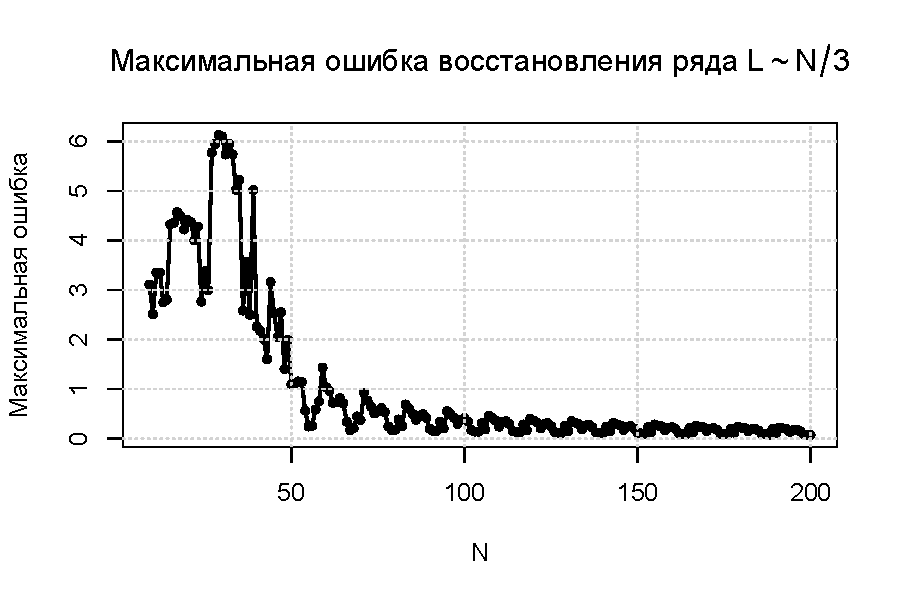
\includegraphics[width=0.85\textwidth]{Pictures/MaxERS.pdf}
			\caption{Максимальные ошибки восстановления ряда в зависимости от длины ряда при $\widetilde{h}_n = n + 3\cos(\pi n/2 + \pi/8)$.}\label{pic:1}
		\end{figure}
		\note{
			Прокомментируем результаты вычислительного эксперимента: по рисунку \ref{pic:1} убедимся, что максимальные по модулю ошибки восстановления ряда стремятся к нулю с ростом N.
		}
	\end{frame}
	\begin{frame}{Приложение. Результаты вычислительных экспериментов}
		\begin{figure}[!h]
			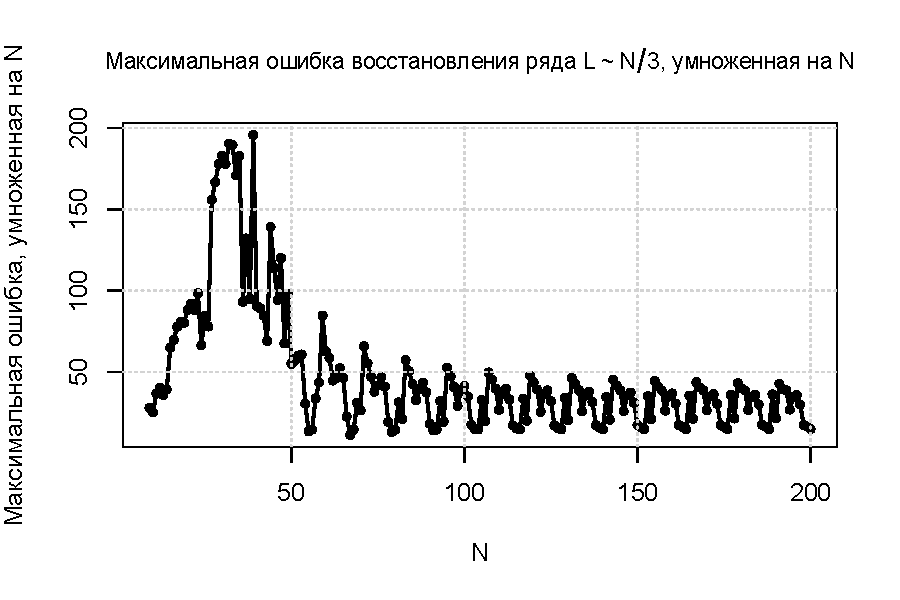
\includegraphics[width=0.85\textwidth]{Pictures/MaxERSNo.pdf}
			\caption{Максимальные ошибки восстановления ряда, умноженные на N, в зависимости от длины ряда N для $\widetilde{h}_n = n + 3\cos(\pi n/2 + \pi/8)$.}\label{pic:2}
		\end{figure}
		\note{
			Рисунок \ref{pic:2} демонстрирует, что после умножения ряда рисунка \ref{pic:1} на N максимальные по модулю ошибки восстановления ряда становятся ограниченными, что подтверждает полученный результат.
		}
	\end{frame}
	
	\begin{frame}{Заключение}
		\begin{enumerate}
			\item Поставлена общая теоретическая задача; 
			\item Дана оценка $\|\mathbf{P}_0^\bot(\delta) - \mathbf{P}_0^\bot - \sum\limits^n_{p=1}\mathbf{W}_p(\delta)\|\;\forall n\in\mathbb{N}$; 
			\item Обобщён результат \cite{ZNekrutkin} асимптотической разделимости линейного сигнала с линейной комбинацией гармоник с $L=K$ до $L/N\rightarrow\alpha\in(0,1)$;
			\item Проведён вычислительный эксперимент, подтверждающий полученный результат. 
		\end{enumerate}
		\note{
			В ходе проделанных работ были изучены теоретические свойства метода SSA, поставлена общая теоретическая задача, дана оценка \textbf{нормы разностей ортогональных проекций с дубль-вэ для произвольного $n$}, обобщён случай асимптотической разделимости линейного сигнала с линейной комбинацией гармоник с $L=K$ до $L/N\rightarrow\alpha\in(0,1)$, а также проведён вычислительный эксперимент, подтверждающий полученный результат. 
		}
	\end{frame}
	
	\begin{frame}{Список литературы}
		\bibliographystyle{ugost2008}
		\bibliography{report_SSA}
		
		\note{
			На данном слайде представлен список основных источников, используемых в моей работе.
			Спасибо за внимание.
		}
	\end{frame}
	
\end{document}
